\documentclass[14pt,a4paper,report]{report}
\usepackage[a4paper, mag=1000, left=2.5cm, right=1cm, top=2cm, bottom=2cm, headsep=0.7cm, footskip=1cm]{geometry}
\usepackage[utf8]{inputenc}
\usepackage[english,russian]{babel}
\usepackage{indentfirst}
\usepackage[dvipsnames]{xcolor}
\usepackage[colorlinks]{hyperref}
\usepackage{listings} 
\usepackage{fancyhdr}
\usepackage{caption}
\usepackage{graphicx}
\hypersetup{
	colorlinks = true,
	linkcolor  = black
}

\usepackage{titlesec}
\titleformat{\chapter}
{\Large\bfseries} % format
{}                % label
{0pt}             % sep
{\huge}           % before-code


\DeclareCaptionFont{white}{\color{white}} 

% Listing description
\usepackage{listings} 
\DeclareCaptionFormat{listing}{\colorbox{gray}{\parbox{\textwidth}{#1#2#3}}}
\captionsetup[lstlisting]{format=listing,labelfont=white,textfont=white}
\lstset{ 
	% Listing settings
	inputencoding = utf8,			
	extendedchars = \true, 
	keepspaces = true, 			  	 % Поддержка кириллицы и пробелов в комментариях
	language = C,            	 	 % Язык программирования (для подсветки)
	basicstyle = \small\sffamily, 	 % Размер и начертание шрифта для подсветки кода
	numbers = left,               	 % Где поставить нумерацию строк (слева\справа)
	numberstyle = \tiny,          	 % Размер шрифта для номеров строк
	stepnumber = 1,               	 % Размер шага между двумя номерами строк
	numbersep = 5pt,              	 % Как далеко отстоят номера строк от подсвечиваемого кода
	backgroundcolor = \color{white}, % Цвет фона подсветки - используем \usepackage{color}
	showspaces = false,           	 % Показывать или нет пробелы специальными отступами
	showstringspaces = false,    	 % Показывать или нет пробелы в строках
	showtabs = false,           	 % Показывать или нет табуляцию в строках
	frame = single,              	 % Рисовать рамку вокруг кода
	tabsize = 2,                  	 % Размер табуляции по умолчанию равен 2 пробелам
	captionpos = t,             	 % Позиция заголовка вверху [t] или внизу [b] 
	breaklines = true,           	 % Автоматически переносить строки (да\нет)
	breakatwhitespace = false,   	 % Переносить строки только если есть пробел
	escapeinside = {\%*}{*)}      	 % Если нужно добавить комментарии в коде
}

\begin{document}

\def\contentsname{Содержание}

% Titlepage
\begin{titlepage}
	\begin{center}
		\textsc{Санкт-Петербургский Политехнический 
			Университет Петра Великого\\[5mm]
			Кафедра компьютерных систем и программных технологий}
		
		\vfill
		
		\textbf{Отчёт по дополнительной работе №1\\[3mm]
			Курс: «Операционные системы»\\[6mm]
			Тема: «Структура контекста процесса»\\[35mm]
		}
	\end{center}
	
	\hfill
	\begin{minipage}{.5\textwidth}
		Выполнил студент:\\[2mm] 
		Бояркин Никита Сергеевич\\
		Группа: 43501/3\\[5mm]
		
		Проверил:\\[2mm] 
		Душутина Елена Владимировна
	\end{minipage}
	\vfill
	\begin{center}
		Санкт-Петербург\\ \the\year\ г.
	\end{center}
\end{titlepage}

% Contents
\tableofcontents
\clearpage

\chapter{Дополнительная работа №1}

\section{Цель работы}

\begin{itemize}
	\item Изучение контекста процесса.
	\item Ознакомление с дескриптором процесса.
	\item Изучение переменных окружения.
\end{itemize}

\section{Программа работы}

\begin{enumerate}
	\item Привести информацию о структуре контекста процесса.
	\item Привести структуру языка \emph{C}, описывающую контекст процесса.
	\item Привести информацию о дескрипторе процесса.
	\item Привести структуру языка \emph{C}, описывающую дескриптор процесса.
	\item Изучить функцию для обработки флагов \emph{getopt}, привести пример программы.
	\item Создать программу, выводящую массив переменных окружения \emph{\_\_environ}.
	\item Получить конкретную переменную окружения функцией \emph{getenv}.
	\item Создать собственную переменную окружения функцией \emph{setenv}, посмотреть изменился ли массив переменных окружения \emph{\_\_environ}.
\end{enumerate}	


\section{Характеристики системы}

Некоторая информация об операционной системе и текущем пользователе:

\lstinputlisting{listings/0.my.log}

Информация об операционной системе и текущем пользователе компьютера в лаборатории:

\lstinputlisting{listings/0.lab.log}

На домашнем и лабораторном компьютерах установлены реальные системы.

\section{Ход работы}

\subsection{Структура контекста процесса}

Контекст процесса включает в себя содержимое адресного пространства задачи, выделенного процессу, а также содержимое относящихся к процессу аппаратных регистров и структур данных ядра. С формальной точки зрения, контекст процесса объединяет в себе пользовательский контекст (user-level context), регистровый контекст (register context) и системный контекст (system-level context).

\subsubsection{Пользовательский контекст}

Пользовательский контекст состоит из команд и данных процесса, стека задачи и содержимого совместно используемого пространства памяти в виртуальных адресах процесса. Те части виртуального адресного пространства процесса, которые периодически отсутствуют в оперативной памяти вследствие выгрузки или замещения страниц, также включаются в пользовательский контекст.

\subsubsection{Регистровый контекст}

Регистровый контекст включает в себя содержимое аппаратных регистров процесса, таких как:

\begin{itemize}
	\item \emph{Счетчик команд (PC)} - указывает на адрес следующей исполняемой команды. Адрес является виртуальным внутри пространства ядра или пространства задачи.
	\item \emph{Регистр состояния процессора (PS)} - указывает на аппаратный статус машины по отношению к процессу. Регистр состояния процессора обычно содержит поля, которые указывают, является ли результат последнего вычисления нулевым, положительным, отрицательным, переполнен ли регистр с установкой бита переноса и др. В других имеющих важное значение полях регистра состояния процессора указывается текущий уровень прерывания процессора, а также текущий и предыдущий режимы выполнения процесса (режим ядра/задачи). По значению поля текущего режима выполнения процесса устанавливается, может ли процесс выполнять привилегированные команды и обращаться к адресному пространству ядра.
	\item \emph{Указатель вершины стека (SP)} - в зависимости от архитектуры машины указатель вершины стека показывает на следующий свободный элемент стека или на последний используемый элемент. От архитектуры машины также зависит направление увеличения стека (к старшим или младшим адресам).
	\item \emph{Регистры общего назначения} - в них содержится информация, сгенерированная процессом во время его выполнения. 
\end{itemize}

\subsubsection{Системный контекст}

Системный контекст процесса имеет статическую и динамическую части. На протяжении всего времени выполнения процесс постоянно располагает единственную статическую часть системного контекста, но может иметь переменное число динамических частей. Динамическую часть системного контекста можно представить в виде стека, элементами которого являются контекстные уровни, которые помещаются в стек ядром или выталкиваются из стека при наступлении различных событий.

Статическая часть системного контекста включает в себя следующие составляющие:

\begin{itemize}
	\item Запись в таблице процессов, описывающая состояние процесса и содержащая различную управляющую информацию, к которой ядро всегда может обратиться. Например, информацию о том, в каком режиме выполняется процесс, приостановлен ли процесс, находится ли в переходном состоянии и др.
	\item Часть адресного пространства задачи, выделенная процессу, где хранится управляющая информация о процессе, доступная только в контексте процесса. Общие управляющие параметры, такие как приоритет процесса, хранятся в таблице процессов, поскольку обращение к ним должно производиться за пределами контекста процесса.
	\item Записи частной таблицы областей процесса, общие таблицы областей и таблицы страниц, необходимые для преобразования виртуальных адресов в физические, в связи с чем в них описываются области команд, данных, стека и другие области, принадлежащие процессу. Если несколько процессов совместно используют общие области, эти области входят составной частью в контекст каждого процесса, поскольку каждый процесс работает с этими областями независимо от других процессов. В задачи управления памятью входит идентификация участков виртуального адресного пространства процесса, не являющихся резидентными в памяти.
\end{itemize}

Динамическая часть системного контекста включает в себя следующие составляющие:

\begin{itemize}
	\item Стек ядра, в котором хранятся записи процедур ядра, если процесс выполняется в режиме ядра. Несмотря на то, что все процессы пользуются одними и теми же программами ядра, каждый из них имеет свою собственную копию стека ядра для хранения индивидуальных обращений к функциям ядра. Пусть, например, один процесс вызывает функцию \emph{creat} и приостанавливается в ожидании назначения нового индекса, а другой процесс вызывает функцию \emph{read} и приостанавливается в ожидании завершения передачи данных с диска в память. Оба процесса обращаются к функциям ядра и у каждого из них имеется в наличии отдельный стек, в котором хранится последовательность выполненных обращений. Ядро должно иметь возможность восстанавливать содержимое стека ядра и положение указателя вершины стека для того, чтобы возобновлять выполнение процесса в режиме ядра. В различных системах стек ядра часто располагается в пространстве процесса, однако этот стек является логически-независимым и, таким образом, может помещаться в самостоятельной области памяти. Когда процесс выполняется в режиме задачи, соответствующий ему стек ядра пуст.
	\item Динамическая часть системного контекста процесса, состоящая из нескольких уровней и имеющая вид стека, который освобождается от элементов в порядке, обратном порядку их поступления. На каждом уровне системного контекста содержится информация, необходимая для восстановления предыдущего уровня и включающая в себя регистровый контекст предыдущего уровня.
\end{itemize}

Ядро помещает контекстный уровень в стек при возникновении прерывания, при обращении к системной функции или при переключении контекста процесса. Контекстный уровень выталкивается из стека после завершения обработки прерывания, при возврате процесса в режим задачи после выполнения системной функции, или при переключении контекста. Таким образом, переключение контекста влечет за собой как помещение контекстного уровня в стек, так и извлечение уровня из стека: ядро помещает в стек контекстный уровень старого процесса, а извлекает из стека контекстный уровень нового процесса. Информация, необходимая для восстановления текущего контекстного уровня, хранится в записи таблицы процессов.

\subsubsection{Компоненты контекста процесса}

На Рисунке 1.1 изображены компоненты контекста процесса. Слева на рисунке изображена статическая часть контекста. В нее входят: пользовательский контекст, состоящий из программ процесса (машинных инструкций), данных, стека и разделяемой памяти (если она имеется), а также статическая часть системного контекста, состоящая из записи таблицы процессов, пространства процесса и записей частной таблицы областей (информации, необходимой для трансляции виртуальных адресов пользовательского контекста). Справа на рисунке изображена динамическая часть контекста. Она имеет вид стека и включает в себя несколько элементов, хранящих регистровый контекст предыдущего уровня и стек ядра для текущего уровня. Нулевой контекстный уровень представляет собой пустой уровень, относящийся к пользовательскому контексту. Стрелка, соединяющая между собой статическую часть системного контекста и верхний уровень динамической части контекста, означает то, что в таблице процессов хранится информация, позволяющая ядру восстанавливать текущий контекстный уровень процесса.

\begin{figure}[h!]
	\centering
	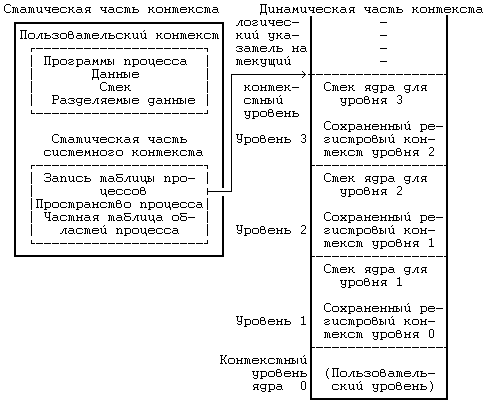
\includegraphics[scale = 1.0]{images/1.png}
	
	\caption{}
	\label{image:1}
\end{figure}

Количество контекстных уровней ограничивается числом поддерживаемых в машине уровней прерывания.

\subsubsection{Структура user}

Контекст процесса формально описан структурой \emph{struct user} в файле \emph{/usr/include/sys/user.h}. Эта структура содержит следующую информацию:

\begin{itemize}
	\item Адрес дескриптора процесса в таблице процессов.
	\item Адрес таблицы открытых файлов процесса.
	\item Адрес таблицы сигналов.
	\item Блок управления процессом.
	\item Текущий каталог процесса.
	\item Корневой каталог процесса.
	\item Виртуальный адрес процедурного сегмента.
	\item Виртуальный адрес сегмента инициализированных данных.
	\item Виртуальный адрес сегмента неинициализированных данных.
\end{itemize}

\subsection{Дескриптор процесса}

Дескриптор процесса содержит такую информацию о процессе, которая необходима ядру в течение всего жизненного цикла процесса, независимо от того, находится ли он в активном или пассивном состоянии, находится ли образ процесса в оперативной памяти или выгружен на диск. Дескрипторы отдельных процессов объединены в список, образующий таблицу процессов. Память для таблицы процессов отводится динамически в области ядра. На основании информации, содержащейся в таблице процессов, операционная система осуществляет планирование и синхронизацию процессов. В дескрипторе прямо или косвенно (через указатели на связанные с ним структуры) может содержаться информация о состоянии процесса, расположении образа процесса в оперативной памяти и на диске, о значении отдельных составляющих приоритета, а также его итоговое значение – глобальный приоритет, идентификатор пользователя, создавшего процесс, информация о родственных процессах, о событиях, осуществления которых ожидает данный процесс и некоторая другая информация.

\subsubsection{Структура proc}

Дескриптор процесса формально описан структурой \emph{struct proc} в заголовочном файле \emph{/usr/include/sys/proc.h}. Основные поля структуры \emph{struct proc} могут быть классифицированы по характеру данных следующим образом:

\begin{itemize}
	
	\item Поля идентификации процесса, такие как: личный идентификатор процесса, идентификатор процесса-предка, идентификатор группы процесса, реальный идентификатор владельца процесса, реальный идентификатор группы владельца процесса, эффективный идентификатор владельца процесса, эффективный идентификатор группы владельца процесса.
	
	\item Поля диспетчеризации процессов, такие как: приоритет процесса, системная составляющая приоритета процесса, пользовательская составляющая приоритета процесса, время нахождения процесса в RAM или в области своппинга.
	
	\item Поля внутренней синхронизации процессов, такие как: статус процесса, идентификатор события, которое ожидает процесс.
	
	\item Поля сигнальной коммуникации процессов, такие как: поле регистрации номеров полученных сигналов, поле регистрации сигналов с отложенной обработкой, номер текущего сигнала, маска номеров игнорируемых сигналов, маска номеров перехваченных сигналов.
	
	\item Поля адресации процесса, такие как: адрес сегментной таблицы процесса, адрес контекста процесса.
	
	\item Поля размеров сегментов процесса, такие как: размер процедурного сегмента образа процесса, размер сегмента данных образа процесса, размер стека образа процесса.
	
	\item Поля ссылок на дескрипторы других процессов, такие как: ссылка на следующий элемент очереди процессов,ссылка на первый элемент очереди процессов, ссылка на последний элемент очереди процессов, ссылка на следующий элемент таблицы процессов, ссылка на дескриптор процесса-предка, ссылка на дескриптор младшего процесса-потомка.
	
	
\end{itemize}

\subsection{Передача опций в программу, функция getopt}

Функция \emph{getopt} разбирает аргументы командной строки. Аргументы \emph{argc} и \emph{argv} являются счетчиком и массивом аргументов, которые передаются функции \emph{main} при запуске программы. Элемент \emph{argv}, начинающийся с $-$, считается опцией. Символы этого элемента (не считая начального $-$) являются символами опций. При каждом повторном вызове \emph{getopt} возвращаются символы следующей опции. 

Если \emph{getopt} находит символ опции, она возвращает этот символ, обновляя внешнюю переменную \emph{optind} и статическую переменную \emph{nextchar}, так что следующий вызов \emph{getopt} может продолжить проверку со следующего символа опции или элемента \emph{argv}. Если символов опций больше нет, то \emph{getopt} возвращает -1.

Третий аргумент функции Если \emph{getopt} является строкой, содержащей допустимые символы опций. Если за таким символом стоит двоеточие, то опция требует указания аргумента. Два двоеточия означают, что опция имеет необязательный аргумент.

Рассмотрим функцию \emph{getopt} на примере тестовой программы:

\lstinputlisting{listings/getopt.c}

Рассмотрим вывод программы с различными опциями:

\lstinputlisting{listings/getopt.log}

Вывод программы значительным образом зависит от того требует ли опция аргумента или нет.

\subsection{Работа с переменными окружения, функции getenv, setenv}

Все переменные окружения хранятся в массиве строк \emph{\_\_environ}, определенном в файле \emph{unistd.h}. Выведем все переменные окружения для тестовой программы:

\lstinputlisting{listings/env.c}

Результат работы программы:

\lstinputlisting{listings/env.log}

Функция доступа к переменным окружения \emph{getenv} возвращает указатель на строку если в качестве аргумента указано имя существующей переменной окружения, если переменная отсутствует, возвращается NULL. Попробуем вывести несколько переменных окружения:

\lstinputlisting{listings/getenv.c}

Результат работы программы:

\lstinputlisting{listings/getenv.log}

Функция \emph{setenv} добавляет новую или изменяет существующую переменную окружения. Если третий аргумент функции не равен нулю, то переменная перезаписывается, в противном случае переменная остается нетронутой, \emph{setenv} возвращает 0 при успешном завершении и -1, если произошла ошибка. Создадим новую переменную окружения и изменим несколько уже существующих:

\lstinputlisting{listings/setenv.c}

Результат работы программы:

\lstinputlisting{listings/setenv.log}

Из результатов работы программы видно, что при добавлении новой переменной окружения функцией \emph{setenv} массив переменных окружения \emph{\_\_environ} также изменился.

\section{Вывод}

В ходе работы была рассмотрена структура контекста процесса в ОС Linux. Контекст принято разделят на три составляющих: регистровый контекст, системный контекст и пользовательский контекст. В составе системного контекста принято выделять статическую и динамические части.

Была рассмотрена функция обработки флагов \emph{getopt}. Функция позволяет задавать аргументы опций, как требующие обязательный аргумент, требующие необязательный аргумент, не требующие аргументов. Это очень удобно использовать при обработке данных из командной строки.

Был рассмотрен массив переменных окружения \emph{\_\_environ}, а также функции для работы с переменными окружения \emph{setenv} и \emph{getenv}. Переменные окружения могут быть использованы для получения информации о языке системы, директории, из которой вызвана программа, терминала, из которого вызвана программа и др.

\section{Список литературы}

\begin{itemize}
	\item Модификация окружения [Электронный ресурс]. — URL: \href{http://www.clinuxworld.com/programming/453-setenv}{http://www.clinuxworld.com/programming/453-setenv} (дата обращения 30.10.2016).
	
	\item Работа с переменными окружения [Электронный ресурс]. — URL: \href{http://www.firststeps.ru/linux/r.php?17}{http://www.firststeps.ru/linux/r.php?17} (дата обращения 30.10.2016).
	
	\item Структура процессов [Электронный ресурс]. — URL: \href{http://khpi-iip.mipk.kharkiv.edu/library/extent/os/bach/bach06.html}{http://khpi-iip.mipk.kharkiv.edu/library/extent/os/ba\linebreak ch/bach06.html} (дата обращения 30.10.2016).
	
	\item Состояние процесса [Электронный ресурс]. — URL: \href{http://citforum.ru/operating_systems/bach/glava_57.shtml}{http://citforum.ru/operating\_systems/bach/glava\_57.s\linebreak html} (дата обращения 30.10.2016).
	
	\item Организация процессов OS UNIX [Электронный ресурс]. — URL: \href{http://cad.narod.ru/methods/os_unix/unibas/process.html}{http://cad.narod.ru/methods/os\_unix/un\linebreak ibas/process.html} (дата обращения 30.10.2016).
	
	\item Контекст процесса [Электронный ресурс]. — URL: \href{http://citforum.ru/operating_systems/bach/glava_59.shtml}{http://citforum.ru/operating\_systems/bach/glava\_59.sh\linebreak tml} (дата обращения 30.10.2016).
	
	\item Мануал getopt [Электронный ресурс]. — URL: \href{https://www.opennet.ru/man.shtml?topic=getopt}{https://www.opennet.ru/man.shtml?topic=getopt} (дата обращения 30.10.2016).
\end{itemize}

\end{document}